\documentclass[10pt,a4paper]{article}

%double si on veut une version prof et une version élève. simple si on veut une seule version.
\newcommand{\buildmode}{double}

\InputIfFileExists{version.tex}{}{}
% Version (définie par le script)
\providecommand{\version}{eleve}

\usepackage{feuilleactivite}

%%%à modifier à chaque fois

\renewcommand{\niveau}{2nde}
\renewcommand{\chapitre}{Équations, solution d'inéquations}
\renewcommand{\numchap}{0.3} 
\renewcommand{\theme}{Nombres et calcul}

\begin{document}

\prof{
    \begin{itemize}
        \item En début de cours, on a fait les fractions décimales remarquables et on les a fait placer sur une droite.
        \item  On peut parler d'abscisse d'un point sur une droite.
    \end{itemize}
   
}

%\legendeicones

\vspace{-0.3cm}

\begin{objectifs}
\begin{itemize}
    \item Comprendre les concepts d'équation et d'inéquation.
    \item Connaître la méthode pour résoudre des équation.
    \item Savoir représenter les solutions d'équations ou d'inéquation sur un axe.
\end{itemize}
\end{objectifs}

\prof{
    Exercice 1 trop difficile ?
}
\section{Equations}
\begin{exo}[][]

Placez les nombres suivant sur l'axe gradué ci-dessous : -2, 0 , \(\dfrac{1}{2}\), \(\dfrac{3}{2}\), \(-\dfrac{7}{3}\), \(\dfrac{21}{5}\).

\vspace{1cm}
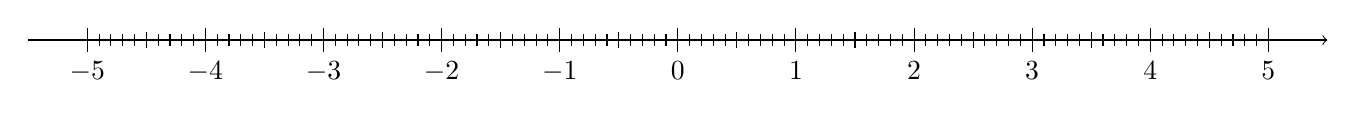
\begin{tikzpicture}[scale=1.5]
\draw[->] (-5.5,0)--(5.5,0);
\foreach \x in {-5,..., 4}{
    \draw (\x,0.1)--(\x,-0.1) node[below] {\(\x\)};
    \draw (\x+0.5,0.07)--(\x+0.5,-0.07) ;
    \foreach \minx in {0.1, 0.2, ..., 0.9}{
        \draw (\x+\minx, 0.05)--(\x+\minx, -0.05);
    }
}
    \draw (5,0.1)--(5,-0.1) node[below] {\(5\)};
\end{tikzpicture}
\end{exo}

\begin{exo}[][]

    Dans chacun des cas ci-dessous, vérifier si le nombre proposé est solution. Sinon, proposer une solution.
    \begin{tasks}(3)
    \task \( x+4 = 10\) \hspace{0.5cm} \(x=5\)
    \task \( 2x-4 = x+1\) \hspace{0.5cm} \(x=5\)
    \task \( 4x = -12\) \hspace{0.5cm} \(x=-3\)
    \task \( 4(x+2) = 12\) \hspace{0.5cm} \(x=3\)
    \task \( 4x = 2\) \hspace{0.5cm} \(x=\dfrac{1}{2}\)
    \task \( 2x  = \dfrac{2}{3}\) \hspace{0.5cm} \(x=\dfrac{1}{4}\)
    \end{tasks}
\end{exo}



\begin{exo}[][]

Résoudre chacune des équations suivantes, puis placer les solutions sur l'axe gradué ci-dessous.

\begin{tasks}(3)
    \task \(x+2=6\)
    \task \(3x-1=8\)
    \task \(x-5=-4\)
    \task \(2x+4=7\)
    \task \(-2x=8\)
    \task \(5x=-1\)
\end{tasks}

\vspace{1cm}
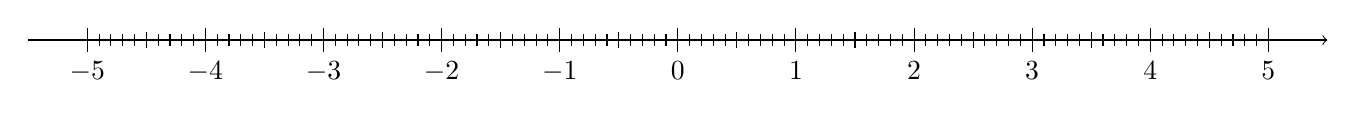
\begin{tikzpicture}[scale=1.5]
\draw[->] (-5.5,0)--(5.5,0);
\foreach \x in {-5,..., 4}{
    \draw (\x,0.1)--(\x,-0.1) node[below] {\(\x\)};
    \draw (\x+0.5,0.07)--(\x+0.5,-0.07) ;
    \foreach \minx in {0.1, 0.2, ..., 0.9}{
        \draw (\x+\minx, 0.05)--(\x+\minx, -0.05);
    }
}
    \draw (5,0.1)--(5,-0.1) node[below] {\(5\)};
\end{tikzpicture}
\end{exo}

\prof{
    L'axe est peut-être perturbant. Est-ce qu'il vaut pas mieux leur faire tracer eux-même ? 
}


\begin{multicols}{2}
    \begin{minipage}{0.45\textwidth}
     \begin{exo}[][]

    $x$ est un nombre positif. Pour quelle valeur de $x$ le périmètre du triangle ci-contre est-il égal à 30 ?
\end{exo}   
    \end{minipage}

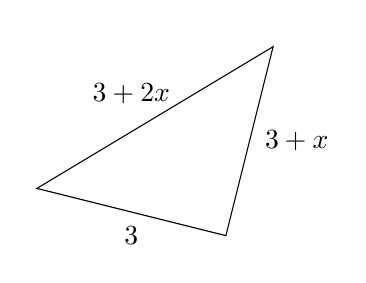
\begin{tikzpicture}[scale=0.6]
\draw (0,0) node[anchor=north]{}
  -- (4,-1) node[anchor=north]{}
  -- (5,3) node[anchor=south]{}
  -- cycle;
\draw (2,-1) node {$3$};
\draw (5.5,1) node {$3+x$};
\draw (2,2) node {$3+2x$};
\end{tikzpicture}
\end{multicols}

\begin{exo}[][appro]
    Un élève de seconde a eu quatre contrôles ce trimestre. Il a eu 10/20 et 15/20 aux deux premiers. Sachant qu'il a obtenu la même note aux contrôles 3 et 4 et que sa moyenne est 14/20, quelles sont ses notes aux  contrôles 3 et 4 ?
\end{exo}

\prof{
    On peut commencer la partie 2 sur les inéquations avant d'entamer le dernier exerice. Si on a le temps, on pourra revenir dessus ensuite.
}
\begin{exo}[][appro]
Résoudre les équations suivantes \begin{tasks}(3)
    \task \(3(x-12)=21\)
    \task \(\dfrac{-x+5}{4}=20\)
    \task \(x^2=9\)
\end{tasks}
\end{exo}

\newpage
\section{Inéquations}

\prof{
    Est-ce qu'on dit "inéquation" pour un encadrement ?

    Pas convaincu par ma question 1
}
\begin{exo}[][]

    On considère \textbf{l'inéquation} \(-2< x\leq 3\) où \(x\) est l'inconnue.
    \begin{enumerate}
        \item Pourquoi dit-on "inéquation" et pas "équation" ?
        \item Lesquels de ces nombres peuvent être une solution de cette inéquation ? \begin{tasks}(3)
            \task \(0\)
            \task \(2,54\)
            \task \(13\%\)
            \task \(4\)
            \task \(\pi\)
            \task \(\dfrac{3}{2}\)
            \task \(3\)
            \task \(-2\)
            \task \(-\dfrac{1}{4}\)
            \task \(\dfrac{11}{2}\)
            \task \(\dfrac{125}{100}\)
        \end{tasks}
        \item Colorer sur la droite graduée l'ensemble des nombres appartenant à l'ensemble précédent.\\
        
        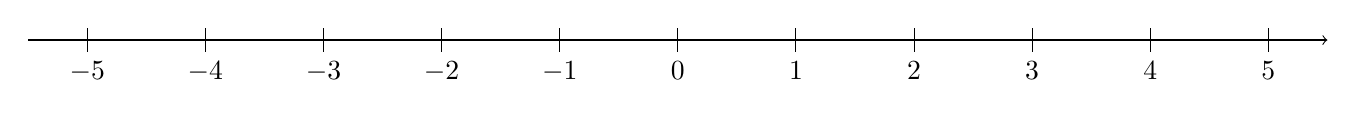
\begin{tikzpicture}[scale=1.5]
        \draw[->] (-5.5,0)--(5.5,0);
        \foreach \x in {-5,..., 5}{
            \draw (\x,0.1)--(\x,-0.1) node[below] {\(\x\)};
        }
        \end{tikzpicture}
    \end{enumerate}
\end{exo}

\begin{exo}[][]

    Représenter sur une droite \underline{graduée} les solutions des inéquations suivantes :
    \begin{enumerate}
        \item \(0\geq x \geq \dfrac{7}{4}\) 
        \vspace{1cm}
        \item \(x \leq -\dfrac{1}{3}\) 
        \vspace{1cm}
        \item \(x > -\dfrac{5}{2}\) 
        \vspace{1cm}
    \end{enumerate}
\end{exo}

\begin{exo}[][]

On peut représenter les solutions d'une inéquation dans des intervalles. Pour chaque inéquation de la colonne de gauche, retrouver l'intervalle dans celle de droite.

\renewcommand{\arraystretch}{2}
\begin{tabular}{rp{0.1cm}cp{2cm}cp{0.1cm}l}
    \(x<-\dfrac{4}{3}\) &  & \(\bullet\) &  & \(\bullet\) & & \(\left]3\ ;\ +\infty\right[\) \\    
    \(x>3\) &  & \(\bullet\) &  & \(\bullet\) & & \([0\ ;\ 2[\) \\
    \(x\geq 3\) &  & \(\bullet\) &  & \(\bullet\) & & \(\left]-\infty\ ;\ \dfrac{4}{3}\right[\) \\
    \(-2< x <2\) &  & \(\bullet\) &  & \(\bullet\) & & \([3\ ;\ +\infty[\) \\
    \(0\leq x < 2\) &  & \(\bullet\) &  & \(\bullet\) & & \(]-2\ ;\ 2[\) \\

    \(0< x \leq 2\) &  & \(\bullet\) &  & \(\bullet\) & & \(]0\ ;\ 2]\) \\
\end{tabular}

\end{exo}


\prof{
    Ecrire dans le cours ensuite. Préparer des exos en plus ?
}
\newpage

\prof{
    Facultatif
}

\section{Distance entre deux nombres. Valeur absolue}

\prof{
    Dans cet exercice, faire un axe. Montrer que cela revient à déterminer une distance entre deux points et à faire une soustration.
}

\begin{exo}
    \begin{enumerate}
        \item Déterminer le nombre d'années pendant lesquelles chacunes des personnes a vécu : Aristote (384 av. J.-C. - 322 av. J.-C.), Marie Curie (1867 - 1934).
        \item Le désert de Qumran, près de la mer morte, a été occupé par les esséniens entre 150 av J.-C. et 68 ap J.-C. Combien d'années ont-ils occupé ce désert ?
        \item Pythagore a vécu 80 ans et il est mort en 480 avant J.-C. En quelle année est-il né ?
    \end{enumerate}
\end{exo}

\begin{exo}

    On a tracé la droite numérique :
    
    \vspace{1cm}
    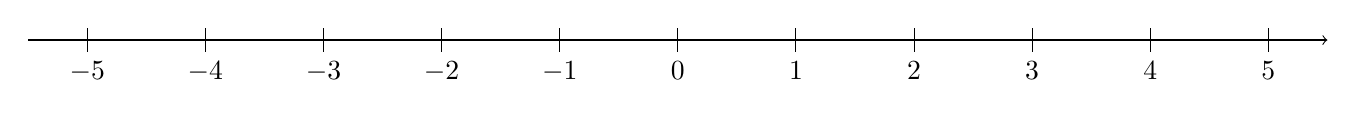
\begin{tikzpicture}[scale=1.5]
    \draw[->] (-5.5,0)--(5.5,0);
    \foreach \x in {-5,..., 4}{
        \draw (\x,0.1)--(\x,-0.1) node[below] {\(\x\)};
    }
        \draw (5,0.1)--(5,-0.1) node[below] {\(5\)};
    \end{tikzpicture}

    \begin{enumerate}
        \item Placer les points A d'abscisse \(-3\) ; B d'abscisse \(1,6\) ; C d'abscisse \(3,4\) et D d'abscisse \(\dfrac{14}{3}\).
        \item Calculer les distances AB, BC, et DA.
    \end{enumerate}

    \prof{
        Propriete (au tableau ou dans le cours) : la distance entre deux nombres \(a\) et \(b\) est \(b-a\) si \(b\geq a\) ou \(a-b\) si \(a\geq b\). On peut aussi dire que la distance est \(|b-a|\).


        Donc \(|b-a|\ = |a-b|\).
    }
\end{exo}

\begin{exo}[][appro]
    Ecrire sous la forme d'un intervalle l'ensemble des nombres \(x\) tels que \begin{tasks}(2)
        \task \(|x-3|<5\)
        \task  \(|x-11|\geq 2\)
        \task  \(|x+12|<2\)
        \task  \(|x|\geq 4\)
        
    \end{tasks}
\end{exo}

\prof{
    Pour l'exercice ci-dessus : \begin{itemize}
        \item faire verbaliser : La distance entre 3 et \(x\) doit être inférieure à 5.
        \item Faire un schéma
        \item Donner les solutions sous la forme d'un intervalle.
    \end{itemize}
}

\begin{exo}[][]
    Essayez d'enlever les valeurs absolues pour finir les calculs suivants : \begin{tasks}(3)
        \task \(|3-5| =\)
        \task  \(|5-3| = \)
        \task  \(|-6| = \)
        \task  \(|34| = \)
        \task  \(-|5| = \)
        \task  \(|3|-|5| = \)
        
    \end{tasks}
\end{exo}


\begin{exo}[Vrai ou Faux ][appro]

    Les propriétés suivantes sont-elles vraies ou fausses ? Justifier votre réponse.
    \begin{enumerate}
        \item Pour tout nombres \(a\) et \(b\), \(|a+b| = |a|+|b|\).
        \item Il existe des nombres \(a\) et \(b\) tels que \(|a+b| = |a|+|b|\).
        \item Pour tout nombre réel \(a\), \(|-a|=|a|\).
    \end{enumerate}
\end{exo}

\end{document}
